\documentclass[11pt]{beamer}
\usetheme{Malmoe}
\usepackage[utf8]{inputenc}
\usepackage{amsmath}
\usepackage{amsfonts}
\usepackage{amssymb}
\usepackage{tikx}
\usepackage{graphicx}
\usepackage{listings}

\author{zach wick \\ zwick@bareo.io}
\title{Making Sense of CORS using web.py}

\begin{document}

\lstset{
  keywordstyle=\color{blue},
  showspaces=false,
  showstringspaces=false,
  basicstyle=\tiny
}

\begin{frame}
  \titlepage
\end{frame}

\begin{frame}{Agenda}
  \begin{itemize}
  \item About the speaker\\
  \item What is CORS\\
  \item Why is CORS useful\\
  \item How does CORS work\\
    \subitem HTTP\\
    \subitem Simple Requests\\
    \subitem Other Requests\\
  \item Worked Example\\
  \item Best Practices\\
  \item Questions (and hopefully answers)
  \end{itemize}
\end{frame}

\begin{frame}{About the Speaker}

\end{frame}
\begin{frame}{What is CORS?}
  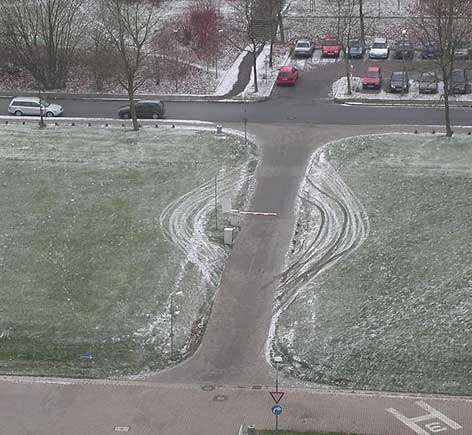
\includegraphics[keepaspectratio=true,width=\framewidth]{circumvent.jpeg}
\end{frame}

\begin{frame}{What is CORS?}
  \begin{columns}[t]
    \begin{column}
      \begin{itemize}
      \item images\\
      \item scripts\\
      \item stylesheets\\
      \item iframes\\
      \item videos\\
      \item some plugin content
      \end{itemize}
    \end{column}
    \begin{column}
      \begin{itemize}
      \item embedded web fonts\\
      \item AJAX
      \end{itemize}
    \end{column}
  \end{columns}
\end{frame}

\begin{frame}{Why is CORS useful?}

\end{frame}
\begin{frame}{How does CORS work?}

\end{frame}

\end{document}
